\section{Matlab Application}
Things to remember for the application:
\begin{itemize}
	\item Information on plots
	\begin{itemize}
		\item Axes titles
		\item Axes labels
	\end{itemize}
	
\end{itemize}

With all the mathematics behind the whole segmentation, feature extraction and classification parts, we realized that instead of having to manually manage each and every function, a more intuitive way of utilizing the whole setup was needed. This lead to the production of a graphical user interface (GUI) consisting of different elements the user could interact with in order to take a piece of sound, segment it and then get an automatic classification. On figure \ref{app-flowchart} a flowchart is provided, presenting the general flow of the application.

\begin{figure}
\begin{center}
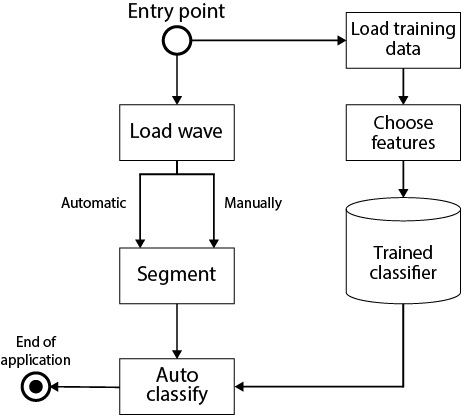
\includegraphics[scale=0.6]{fig/Application_flowchart.png}
\caption{Flowchart of the application.}
\label{app-flowchart}
\end{center}
\end{figure}

\paragraph{Application Workflow} \hspace{0pt} \\
To use the application the thing to do after starting it is to load a waveform of some recording of a person beatboxing, be it you or someone else. This waveform then has to be segmented to identify the points at which each beatboxing sound (e.g. a kick drum or hi-hat) starts and ends. This process can either be done manually by the user or it can automatically be done with the in-built segmentation algorithm. The manual process of segmenting the waveform has to done in an external program such as Sonic Visualiser (http://www.sonicvisualiser.org/) and then loaded into our application.

Before classifying these segments, the classifier has to be trained. To do this we start by loading a dataset that has been manually segmented. This dataset is a recording of multiple instances of the different beatboxing sounds used for the classification. When this dataset is loaded and segmented, the user must choose which features to use during the classification process. As an example we could choose MFCC using an analysis window size of 16 ms and a window skip of 8 ms. The classifier will then analyse all segments in the training dataset based on their MFCC and then store these analysis results to use them when classifying the unknown waveform.

When the user query a classification of the input waveform the classifier will take each segment from the input and compare it to the stored training data. Each segment will through this process get an annotation, i.e. a classification id, telling the user what kind of sound that segment has been interpreted as. A sequence of these annotation could be:

\begin{center}
k k k hh k s
\end{center}

, where the three first segments are classified as kicks followed by a hi-hat and then a snare.

Hereafter the user can try and adjust chosen features or choose new features to train the classifier again and/or a new waveform can be loaded into the application and segmented also to be classified.